% ============================================================
% 讲义 — 人教版七年级下册 第5章 相交线与平行线
% 编译命令：xelatex -interaction=nonstopmode 第5章_相交线与平行线.tex
% ============================================================
\documentclass[12pt, a4paper]{ctexart}
\usepackage[margin=2.2cm]{geometry}
\usepackage{amsmath, amssymb}
\usepackage{enumitem}
\usepackage{tcolorbox}
\usepackage{booktabs}
\usepackage{array}
\usepackage{fancyhdr}
\usepackage{xcolor}
\usepackage{tikz}
\usepackage{hyperref}
\usepackage{graphicx}
\usepackage{multirow}
\usepackage{pgfplots}
\pgfplotsset{compat=1.18}

% 颜色定义
\definecolor{mainblue}{RGB}{41, 98, 168}
\definecolor{lightblue}{RGB}{230, 240, 255}
\definecolor{tipgreen}{RGB}{34, 139, 87}
\definecolor{lightgreen}{RGB}{235, 250, 240}
\definecolor{warnred}{RGB}{200, 50, 50}
\definecolor{lightred}{RGB}{255, 240, 240}
\definecolor{examorange}{RGB}{210, 120, 20}
\definecolor{lightorange}{RGB}{255, 248, 235}
\definecolor{apppurple}{RGB}{120, 60, 170}
\definecolor{lightpurple}{RGB}{245, 238, 255}

% 页眉页脚
\pagestyle{fancy}
\fancyhf{}
\fancyhead[L]{\small\textcolor{mainblue}{\textbf{人教版七年级下册 · 第5章}}}
\fancyhead[R]{\small\textcolor{mainblue}{相交线与平行线讲义}}
\fancyfoot[C]{\small —\ \thepage\ —}
\renewcommand{\headrulewidth}{0.6pt}
\renewcommand{\headrule}{\hbox to\headwidth{\color{mainblue}\leaders\hrule height \headrulewidth\hfill}}
\renewcommand{\footrulewidth}{0pt}

% tcolorbox 样式
\newtcolorbox{knowledgebox}[1][]{%
  colback=lightblue, colframe=mainblue,
  fonttitle=\bfseries\large, title=#1,
  arc=3mm, boxrule=0.8pt,
  left=8pt, right=8pt, top=6pt, bottom=6pt
}

\newtcolorbox{tipbox}[1][]{%
  colback=lightgreen, colframe=tipgreen,
  fonttitle=\bfseries, title=#1,
  arc=2mm, boxrule=0.6pt,
  left=6pt, right=6pt, top=4pt, bottom=4pt
}

\newtcolorbox{warnbox}[1][]{%
  colback=lightred, colframe=warnred,
  fonttitle=\bfseries, title=#1,
  arc=2mm, boxrule=0.6pt,
  left=6pt, right=6pt, top=4pt, bottom=4pt
}

\newtcolorbox{examplebox}[1][]{%
  colback=lightorange, colframe=examorange,
  fonttitle=\bfseries, title=#1,
  arc=3mm, boxrule=0.8pt,
  left=8pt, right=8pt, top=6pt, bottom=6pt
}

\newtcolorbox{appbox}[1][]{%
  colback=lightpurple, colframe=apppurple,
  fonttitle=\bfseries, title=#1,
  arc=3mm, boxrule=0.8pt,
  left=8pt, right=8pt, top=6pt, bottom=6pt
}

\setCJKmainfont{Hiragino Sans GB}
\setCJKsansfont{Heiti SC}

\begin{document}

% ============ 标题页 ============
\begin{center}
{\Huge\bfseries\textcolor{mainblue}{第5章\quad 相交线与平行线}}\\[12pt]
{\Large\textcolor{gray}{讲\quad 义}}\\[8pt]
\rule{0.6\textwidth}{1pt}\\[8pt]
{\normalsize 适用：人教版\quad 七年级下册\quad |\quad 课时：6课时}
\end{center}
\vspace{10pt}

% =============================================================
% 第一部分：知识点讲解
% =============================================================
\section*{\textcolor{mainblue}{一、知识点讲解}}

\subsection*{5.1\quad 相交线}

% ----- 对顶角与邻补角 -----
\begin{knowledgebox}[1.\quad 对顶角与邻补角]
两条直线相交，形成四个角。如图所示，直线 $AB$ 与 $CD$ 相交于点 $O$：

\begin{center}
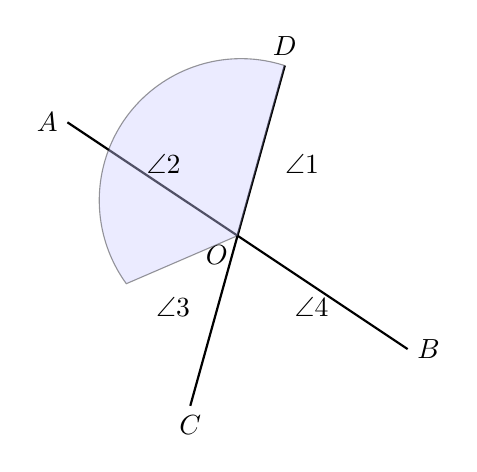
\begin{tikzpicture}[scale=1.2]
  \coordinate (O) at (0,0);
  \coordinate (A) at (-1.8,1.2);
  \coordinate (B) at (1.8,-1.2);
  \coordinate (C) at (-0.5,-1.8);
  \coordinate (D) at (0.5,1.8);
  \draw[thick] (A) -- (B);
  \draw[thick] (C) -- (D);
  \node[below left] at (O) {$O$};
  \node[left] at (A) {$A$};
  \node[right] at (B) {$B$};
  \node[below] at (C) {$C$};
  \node[above] at (D) {$D$};
  % 标记对顶角
  \draw[fill=blue!20, opacity=0.4] (O) -- (0.5,1.8) arc (72:216:1.5) -- cycle;
  \node[above right] at (0.4,0.55) {$\angle 1$};
  \node[below left] at (-0.4,-0.55) {$\angle 3$};
  \node[above left] at (-0.5,0.55) {$\angle 2$};
  \node[below right] at (0.5,-0.55) {$\angle 4$};
\end{tikzpicture}
\end{center}

\textbf{对顶角}：有公共顶点，两边互为反向延长线的两个角。
\begin{itemize}[leftmargin=2em]
  \item \textbf{对顶角相等}。即 $\angle 1 = \angle 3$，$\angle 2 = \angle 4$。
\end{itemize}

\textbf{邻补角}：有公共顶点和一条公共边，另一条边互为反向延长线的两个角。
\begin{itemize}[leftmargin=2em]
  \item \textbf{邻补角互补}。即 $\angle 1 + \angle 2 = 180°$。
\end{itemize}
\end{knowledgebox}

\begin{tipbox}[识别技巧]
\begin{itemize}[leftmargin=2em]
  \item 对顶角：形如"\textbf{X}"交叉，不相邻，相等。
  \item 邻补角：形如"\textbf{L}"靠在一起，相邻，互补（和为 $180°$）。
  \item 对顶角一定成对出现，一个角有两个对顶角是错误说法（一个角只有一对对顶角）。
\end{itemize}
\end{tipbox}

% ----- 垂线 -----
\begin{knowledgebox}[2.\quad 垂线及其性质]
当两条直线相交所成的四个角中，有一个角是直角（$90°$）时，这两条直线互相垂直。

\begin{center}
\begin{tikzpicture}[scale=1.1]
  \coordinate (O) at (0,0);
  \draw[thick] (-2.5,0) -- (2.5,0);
  \draw[thick] (0,-2) -- (0,2);
  \draw (0.3,0) -- (0.3,0.3) -- (0,0.3);
  \node[below] at (0,0) {$O$};
  \node[left] at (-2.5,0) {$A$};
  \node[right] at (2.5,0) {$B$};
  \node[below] at (0,-2) {$C$};
  \node[above] at (0,2) {$D$};
  \node[above right] at (0.15,0.15) {$90°$};
\end{tikzpicture}
\end{center}

记作 $AB \perp CD$，垂足为 $O$。

\textbf{垂线的性质}：
\begin{enumerate}[leftmargin=2em]
  \item \textbf{过一点有且只有一条直线与已知直线垂直。}
  \item \textbf{连接直线外一点与直线上各点的所有线段中，垂线段最短。}
\end{enumerate}

\textbf{点到直线的距离}：从直线外一点到这条直线的\textbf{垂线段的长度}，叫做点到直线的距离。
\end{knowledgebox}

\begin{warnbox}[易错提醒]
\begin{itemize}[leftmargin=2em]
  \item "垂线"是\textbf{直线}，不能说"垂线段最短等于垂线最短"。
  \item 点到直线的距离是一个\textbf{数量}（长度），不是垂线段本身。
  \item 过一点作已知直线的垂线，这个点可以在直线上，也可以在直线外。
\end{itemize}
\end{warnbox}

% ----- 同位角、内错角、同旁内角 -----
\begin{knowledgebox}[3.\quad 同位角、内错角、同旁内角]
当两条直线被第三条直线（截线）所截时，会形成八角关系：

\begin{center}
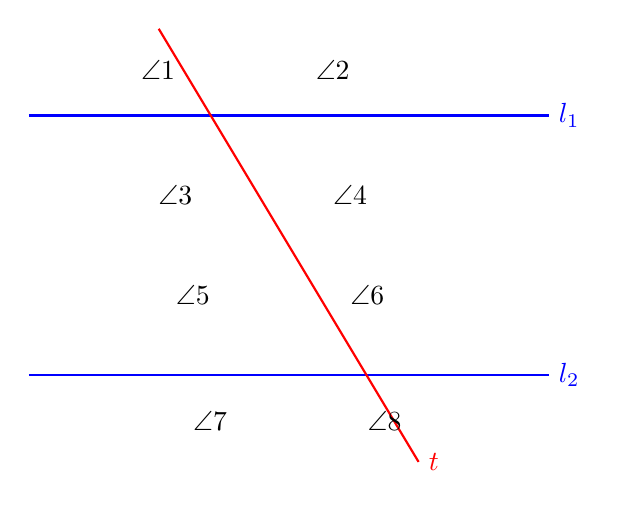
\begin{tikzpicture}[scale=1.1]
  \coordinate (A) at (-3, 1.5);
  \coordinate (B) at (3, 1.5);
  \coordinate (C) at (-3,-1.5);
  \coordinate (D) at (3,-1.5);
  \coordinate (E) at (-1.5, 2.5);
  \coordinate (F) at (1.5,-2.5);
  \draw[thick, blue] (A) -- (B) node[right]{$l_1$};
  \draw[thick, blue] (C) -- (D) node[right]{$l_2$};
  \draw[thick, red] (E) -- (F) node[right]{$t$};
  \node[above left] at (-1.2,1.8) {$\angle 1$};
  \node[above right] at (0.2,1.8) {$\angle 2$};
  \node[below left] at (-1.0,0.8) {$\angle 3$};
  \node[below right] at (0.4,0.8) {$\angle 4$};
  \node[above left] at (-0.8,-0.8) {$\angle 5$};
  \node[above right] at (0.6,-0.8) {$\angle 6$};
  \node[below left] at (-0.6,-1.8) {$\angle 7$};
  \node[below right] at (0.8,-1.8) {$\angle 8$};
\end{tikzpicture}
\end{center}

\begin{itemize}[leftmargin=2em]
  \item \textbf{同位角}：在截线同侧、且在被截两线同侧的一对角。如 $\angle 1$ 与 $\angle 5$，$\angle 2$ 与 $\angle 6$。形如字母"\textbf{F}"。
  \item \textbf{内错角}：在截线两侧、且在被截两线之间的一对角。如 $\angle 3$ 与 $\angle 5$，$\angle 4$ 与 $\angle 6$。形如字母"\textbf{Z}"。
  \item \textbf{同旁内角}：在截线同侧、且在被截两线之间的一对角。如 $\angle 3$ 与 $\angle 6$，$\angle 4$ 与 $\angle 5$。形如字母"\textbf{U}"。
\end{itemize}
\end{knowledgebox}

\subsection*{5.2\quad 平行线及其判定}

% ----- 平行公理 -----
\begin{knowledgebox}[4.\quad 平行公理及推论]
\textbf{平行公理}：经过直线外一点，\textbf{有且只有一条直线}与这条直线平行。

\textbf{推论（平行线的传递性）}：如果两条直线都与第三条直线平行，那么这两条直线也互相平行。
\[
\text{若}\ a \parallel b,\  b \parallel c,\ \text{则}\ a \parallel c。
\]
\end{knowledgebox}

% ----- 平行线的判定 -----
\begin{knowledgebox}[5.\quad 平行线的判定方法]
两条直线被第三条直线所截，可用以下方法判定两直线平行：

\begin{center}
\begin{tikzpicture}[scale=0.9]
  \coordinate (A) at (-3, 1.2);
  \coordinate (B) at (4, 1.2);
  \coordinate (C) at (-3,-1.2);
  \coordinate (D) at (4,-1.2);
  \coordinate (E) at (-1, 2.8);
  \coordinate (F) at (1,-2.8);
  \draw[thick, blue] (A) -- (B);
  \draw[thick, blue] (C) -- (D);
  \draw[thick, red] (E) -- (F);
  \node[right] at (B) {$l_1$};
  \node[right] at (D) {$l_2$};
  \node[right] at (F) {$t$};
  \draw[fill=green!20] (0,1.2) -- (0.5,1.2) arc(0:56:0.5) -- cycle;
  \node at (0.4,1.5) {\small $\alpha$};
  \draw[fill=green!20] (0.667,-1.2) -- (1.167,-1.2) arc(0:56:0.5) -- cycle;
  \node at (1.067,-0.9) {\small $\beta$};
  \node[above] at (0,1.5) {};
\end{tikzpicture}
\end{center}

\begin{enumerate}[leftmargin=2em]
  \item \textbf{同位角相等，两直线平行}：若 $\angle\alpha = \angle\beta$（同位角），则 $l_1 \parallel l_2$。
  \item \textbf{内错角相等，两直线平行}：若内错角相等，则 $l_1 \parallel l_2$。
  \item \textbf{同旁内角互补，两直线平行}：若同旁内角之和为 $180°$，则 $l_1 \parallel l_2$。
\end{enumerate}
\end{knowledgebox}

\begin{tipbox}[判定定理的记忆口诀]
\textbf{判定}平行线（由角推平行）：
\begin{itemize}[leftmargin=2em]
  \item 同位角\textbf{相等} $\Rightarrow$ 平行
  \item 内错角\textbf{相等} $\Rightarrow$ 平行
  \item 同旁内角\textbf{互补} $\Rightarrow$ 平行
\end{itemize}
记住：\textbf{"相等判平行，互补也判平行"}
\end{tipbox}

\subsection*{5.3\quad 平行线的性质}

\begin{knowledgebox}[6.\quad 平行线的性质]
当两条平行线被第三条直线所截时：

\begin{enumerate}[leftmargin=2em]
  \item \textbf{两直线平行，同位角相等。}
  \item \textbf{两直线平行，内错角相等。}
  \item \textbf{两直线平行，同旁内角互补。}
\end{enumerate}

\textbf{注意}：平行线的\textbf{性质}与\textbf{判定}是互逆关系！
\begin{itemize}[leftmargin=2em]
  \item 判定：\textbf{角的关系} $\Rightarrow$ \textbf{平行}
  \item 性质：\textbf{平行} $\Rightarrow$ \textbf{角的关系}
\end{itemize}
\end{knowledgebox}

\begin{warnbox}[易错提醒：判定与性质的区别]
\begin{itemize}[leftmargin=2em]
  \item 看到"\textbf{因为同位角相等，所以两直线平行}"——这是\textbf{判定}。
  \item 看到"\textbf{因为两直线平行，所以同位角相等}"——这是\textbf{性质}。
  \item 判定和性质的\textbf{因果关系正好相反}，使用时不能混淆！
\end{itemize}
\end{warnbox}

% =============================================================
% 第二部分：例题精讲
% =============================================================
\section*{\textcolor{examorange}{二、例题精讲}}

\begin{examplebox}[【例题1】对顶角与邻补角的基本计算]
两条直线相交，$\angle 1$ 与 $\angle 2$ 是对顶角，$\angle 1$ 与 $\angle 3$ 是邻补角。若 $\angle 1 = 70°$，求 $\angle 2$ 和 $\angle 3$。
\end{examplebox}

\textbf{解}：

因为 $\angle 1$ 与 $\angle 2$ 是对顶角，对顶角相等，所以 $\angle 2 = \angle 1 = 70°$。

因为 $\angle 1$ 与 $\angle 3$ 是邻补角，邻补角互补，所以 $\angle 3 = 180° - \angle 1 = 180° - 70° = 110°$。

\begin{tipbox}[方法总结]
邻补角和对顶角的计算，关键是分清两角之间的关系：对顶角相等，邻补角互补（和为 $180°$）。
\end{tipbox}

\vspace{6pt}

\begin{examplebox}[【例题2】垂线与点到直线的距离]
如图，$AB \perp l$ 于点 $B$，$AC \perp l$ 于点 $C$，$AB = 3\text{ cm}$，$AC = 5\text{ cm}$。点 $A$ 到直线 $l$ 的距离是多少？
\end{examplebox}

\begin{center}
\begin{tikzpicture}[scale=1.0]
  \draw[thick] (-2,0) -- (5,0) node[right]{$l$};
  \coordinate (A) at (1.5, 3);
  \coordinate (B) at (1.5, 0);
  \coordinate (C) at (3.5, 0);
  \draw[thick] (A) -- (B) node[midway, left]{$3$};
  \draw[thick] (A) -- (C) node[midway, right]{$5$};
  \draw (1.8,0) -- (1.8,0.3) -- (1.5,0.3);
  \draw (3.8,0) -- (3.8,0.3) -- (3.5,0.3);
  \node[above] at (A) {$A$};
  \node[below] at (B) {$B$};
  \node[below] at (C) {$C$};
\end{tikzpicture}
\end{center}

\textbf{解}：

点到直线的距离是从该点到直线的\textbf{垂线段的长度}。

因为 $AB \perp l$，$AC \perp l$，但 $AB$ 与 $AC$ 是从同一点 $A$ 到直线 $l$ 的两条线段。

根据垂线的性质，过一点有且只有一条直线与已知直线垂直，所以 $B$ 与 $C$ 应为同一点（即 $AC$ 并不垂直于 $l$，题目应理解为 $B$ 为垂足）。

因此，点 $A$ 到直线 $l$ 的距离为 $AB = 3\text{ cm}$。

\vspace{6pt}

\begin{examplebox}[【例题3】同位角、内错角、同旁内角的识别]
如图，直线 $a$，$b$ 被直线 $c$ 所截。找出图中所有的同位角、内错角和同旁内角。
\end{examplebox}

\begin{center}
\begin{tikzpicture}[scale=1.0]
  \coordinate (A) at (-3, 1.5);
  \coordinate (B) at (4, 1.5);
  \coordinate (C) at (-3,-1.5);
  \coordinate (D) at (4,-1.5);
  \coordinate (E) at (-1.5, 3);
  \coordinate (F) at (1.5,-3);
  \draw[thick] (A) -- (B) node[right]{$a$};
  \draw[thick] (C) -- (D) node[right]{$b$};
  \draw[thick] (E) -- (F) node[below]{$c$};
  \node[above left] at (-1.0,1.9) {\small 1};
  \node[above right] at (0.0,1.9) {\small 2};
  \node[below left] at (-0.8,0.7) {\small 3};
  \node[below right] at (0.2,0.7) {\small 4};
  \node[above left] at (-0.4,-0.7) {\small 5};
  \node[above right] at (0.6,-0.7) {\small 6};
  \node[below left] at (-0.2,-1.9) {\small 7};
  \node[below right] at (0.8,-1.9) {\small 8};
\end{tikzpicture}
\end{center}

\textbf{解}：
\begin{itemize}[leftmargin=2em]
  \item \textbf{同位角}：$\angle 1$ 与 $\angle 5$，$\angle 2$ 与 $\angle 6$，$\angle 3$ 与 $\angle 7$，$\angle 4$ 与 $\angle 8$。
  \item \textbf{内错角}：$\angle 3$ 与 $\angle 5$，$\angle 4$ 与 $\angle 6$。
  \item \textbf{同旁内角}：$\angle 3$ 与 $\angle 6$，$\angle 4$ 与 $\angle 5$。
\end{itemize}

\begin{tipbox}[方法总结]
识别三类角的方法：先找截线（公共边所在的直线），再看角在截线的同侧还是两侧，最后看角在两线之间还是之外。
\end{tipbox}

\vspace{6pt}

\begin{examplebox}[【例题4】利用平行线的判定证明平行]
如图，已知 $\angle 1 = \angle 2$。求证：$AB \parallel CD$。
\end{examplebox}

\begin{center}
\begin{tikzpicture}[scale=1.0]
  \coordinate (A) at (-3.5, 1.2);
  \coordinate (B) at (3.5, 1.2);
  \coordinate (C) at (-3.5,-1.2);
  \coordinate (D) at (3.5,-1.2);
  \coordinate (E) at (-1.5, 2.8);
  \coordinate (F) at (0.5,-2.8);
  \draw[thick] (A) -- (B) node[right]{$B$};
  \draw[thick] (C) -- (D) node[right]{$D$};
  \draw[thick] (E) -- (F);
  \node[above left] at (-3.5,1.2) {$A$};
  \node[below left] at (-3.5,-1.2) {$C$};
  \node[above left] at (-1.5,2.8) {$E$};
  \node[below right] at (0.5,-2.8) {$F$};
  \node[above left] at (-0.9,1.7) {\small $\angle 1$};
  \node[above right] at (0.1,1.7) {\small $\angle 2$};
\end{tikzpicture}
\end{center}

\textbf{证明}：

因为 $\angle 1 = \angle 2$（已知），

而 $\angle 1$ 与 $\angle 2$ 是直线 $AB$、$CD$ 被截线 $EF$ 所截形成的\textbf{同位角}，

所以 $AB \parallel CD$（同位角相等，两直线平行）。

\vspace{6pt}

\begin{examplebox}[【例题5】平行线性质与判定的综合]
如图，已知 $AB \parallel CD$，$\angle 1 = 65°$，$\angle 2 = 35°$。求 $\angle BEC$ 的度数。
\end{examplebox}

\begin{center}
\begin{tikzpicture}[scale=1.1]
  \coordinate (A) at (-3, 1);
  \coordinate (B) at (3, 1);
  \coordinate (C) at (-3,-1);
  \coordinate (D) at (3,-1);
  \coordinate (E) at (0, 1);
  \coordinate (F) at (0,-1);
  \coordinate (G) at (0.5, 2);
  \coordinate (H) at (0.5,-2);
  \draw[thick] (A) -- (B) node[right]{$B$};
  \draw[thick] (C) -- (D) node[right]{$D$};
  \node[left] at (A) {$A$};
  \node[left] at (C) {$C$};
  \coordinate (P) at (-1.5, 2.2);
  \coordinate (Q) at (1.0, -2.2);
  \draw[thick] (P) -- (Q);
  \node[above left] at (P) {$P$};
  \node[below right] at (Q) {$Q$};
  \coordinate (Ept) at (-0.25,1);
  \coordinate (Fpt) at (0.5,-1);
  \node[above] at (Ept) {$E$};
  \node[below] at (Fpt) {$F$};
  \node[above left] at (-1.0,1.5) {\small $\angle 1=65°$};
  \node[below right] at (0.2,-1.5) {\small $\angle 2=35°$};
\end{tikzpicture}
\end{center}

\textbf{解}：

因为 $AB \parallel CD$（已知），

过点 $E$ 作 $EF \parallel AB$（平行公理，过直线外一点有且只有一条直线与已知直线平行），

则 $EF \parallel CD$（平行线的传递性）。

因为 $AB \parallel EF$，$\angle 1 = 65°$，

所以 $\angle BEF = \angle 1 = 65°$（两直线平行，内错角相等）。

因为 $EF \parallel CD$，$\angle 2 = 35°$，

所以 $\angle FEC = \angle 2 = 35°$（两直线平行，内错角相等）。

因此 $\angle BEC = \angle BEF + \angle FEC = 65° + 35° = 100°$。

\begin{tipbox}[方法总结]
当题目中出现两条平行线之间的角时，常常需要\textbf{作辅助平行线}来"搬运"角度。这是平行线问题中最常用的技巧。
\end{tipbox}

\vspace{6pt}

\begin{examplebox}[【例题6】判定与性质的综合证明]
如图，已知 $\angle 1 = \angle 2$，$\angle 3 = \angle 4$。求证：$AB \parallel CD$。
\end{examplebox}

\begin{center}
\begin{tikzpicture}[scale=1.0]
  \coordinate (A) at (-3.5, 1.2);
  \coordinate (B) at (3.5, 1.2);
  \coordinate (C) at (-3.5,-1.2);
  \coordinate (D) at (3.5,-1.2);
  \coordinate (E) at (0,0);
  \coordinate (P) at (-2, 2.8);
  \coordinate (Q) at (2, -2.8);
  \draw[thick] (A) -- (B);
  \draw[thick] (C) -- (D);
  \draw[thick] (P) -- (Q);
  \node[left] at (A) {$A$};
  \node[right] at (B) {$B$};
  \node[left] at (C) {$C$};
  \node[right] at (D) {$D$};
  \node[left] at (P) {$E$};
  \node[right] at (Q) {$F$};
  \node[above left] at (-1.2,1.7) {\small $\angle 1$};
  \node[above right] at (0.2,1.7) {\small $\angle 2$};
  \node[below left] at (-0.6,-0.7) {\small $\angle 3$};
  \node[below right] at (0.6,-0.7) {\small $\angle 4$};
\end{tikzpicture}
\end{center}

\textbf{证明}：

因为 $\angle 1 = \angle 2$（已知），

所以 $AE \parallel BF$（同位角相等，两直线平行）。

因为 $\angle 3 = \angle 4$（已知），

所以 $BF \parallel CD$（内错角相等，两直线平行）。

因为 $AE \parallel BF$，$BF \parallel CD$，

所以 $AE \parallel CD$（平行线的传递性），

即 $AB \parallel CD$。

\vspace{6pt}

\begin{examplebox}[【例题7】易错辨析——判定与性质混用]
判断对错：已知 $AB \parallel CD$，$\angle 1 = \angle 2$，所以 $EF \parallel GH$。其中 $\angle 1$ 是 $AB$ 与 $EF$ 被截线所成的同位角，$\angle 2$ 是 $CD$ 与 $GH$ 被截线所成的同位角。这种说法对吗？
\end{examplebox}

\textbf{解}：

这种说法\textbf{不对}。

理由：虽然 $AB \parallel CD$，$\angle 1 = \angle 2$，但 $\angle 1$ 和 $\angle 2$ 并不是 $EF$ 和 $GH$ 被同一条截线所截形成的角。

$\angle 1$ 是 $AB$ 与 $EF$ 的角，$\angle 2$ 是 $CD$ 与 $GH$ 的角。要判断 $EF \parallel GH$，需要 $EF$ 与 $GH$ 被第三条线所截时的同位角（或内错角、同旁内角）关系。

\begin{warnbox}[关键提醒]
使用判定定理时，必须确认是\textbf{两条直线被第三条直线所截}形成的角。不同直线被不同截线所截的角之间没有直接的判定关系。
\end{warnbox}

% =============================================================
% 第三部分：应用题
% =============================================================
\section*{\textcolor{apppurple}{三、应用题}}

\begin{appbox}[【应用1】测量中的垂直与距离]
小明要测量学校旗杆底部 $A$ 到对面围墙的距离。他在地面上找到一点 $P$，使 $AP \perp$ 围墙于点 $B$。他量得 $PB = 12\text{ m}$，$AB = 5\text{ m}$。请问点 $P$ 到围墙的距离是多少？旗杆底部到围墙的距离是多少？
\end{appbox}

\textbf{解}：

\begin{itemize}[leftmargin=2em]
  \item 点 $P$ 到围墙的距离就是 $P$ 到围墙的垂线段的长度。因为 $AP \perp$ 围墙于 $B$，所以 $PB = 12\text{ m}$ 就是点 $P$ 到围墙的垂线段长度，即点 $P$ 到围墙的距离为 $\boxed{12\text{ m}}$。
  \item 旗杆底部 $A$ 到围墙的距离就是 $AB = 5\text{ m}$（因为 $AB \perp$ 围墙）。
\end{itemize}

\vspace{6pt}

\begin{appbox}[【应用2】平行线在道路设计中的应用]
城市规划中，两条主干道 $AB$ 和 $CD$ 互相平行。一条斜路 $EF$ 分别与 $AB$、$CD$ 相交。已知 $\angle AEF = 120°$，求 $\angle EFC$ 的度数。
\end{appbox}

\begin{center}
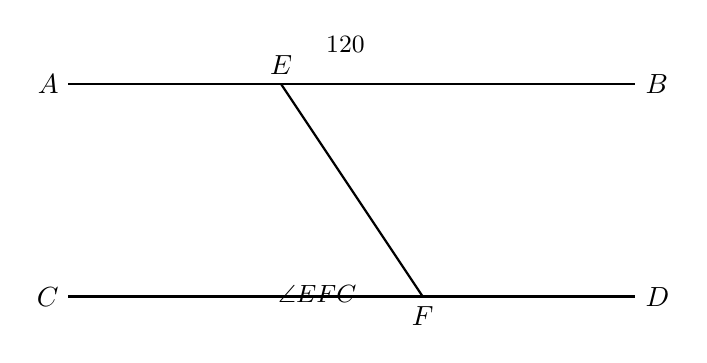
\begin{tikzpicture}[scale=0.9]
  \coordinate (A) at (-4, 1.5);
  \coordinate (B) at (4, 1.5);
  \coordinate (C) at (-4,-1.5);
  \coordinate (D) at (4,-1.5);
  \coordinate (E) at (-1, 1.5);
  \coordinate (F) at (1,-1.5);
  \draw[thick] (A) -- (B) node[right]{$B$};
  \draw[thick] (C) -- (D) node[right]{$D$};
  \draw[thick] (E) -- (F);
  \node[left] at (A) {$A$};
  \node[left] at (C) {$C$};
  \node[above] at (E) {$E$};
  \node[below] at (F) {$F$};
  \node[above right] at (-0.5,1.8) {\small $120°$};
  \node[below left] at (0.2,-1.2) {\small $\angle EFC$};
\end{tikzpicture}
\end{center}

\textbf{解}：

因为 $AB \parallel CD$（已知），

$EF$ 是截线，$\angle AEF$ 与 $\angle EFC$ 是两平行线被 $EF$ 所截形成的\textbf{同旁内角}。

所以 $\angle AEF + \angle EFC = 180°$（两直线平行，同旁内角互补）。

因此 $\angle EFC = 180° - 120° = \boxed{60°}$。

\vspace{6pt}

\begin{appbox}[【应用3】折纸中的平行线问题]
将一张长方形纸片 $ABCD$ 沿 $EF$ 折叠，使点 $A$ 落在 $A'$ 处。已知 $AB \parallel CD$，$\angle AEF = 70°$。求 $\angle A'ED$ 的度数。
\end{appbox}

\textbf{解}：

折叠时 $\angle AEF = \angle A'EF = 70°$（折叠不改变角的大小）。

所以 $\angle AEA' = \angle AEF + \angle A'EF = 70° + 70° = 140°$。

因为 $\angle AEF + \angle BEF = 180°$（$A$、$E$、$B$ 共线），

所以 $\angle BEF = 180° - 70° = 110°$。

因为 $\angle A'EF = 70°$，

$\angle A'ED = 180° - \angle AEF - \angle A'EF$。

注意 $A$、$E$、$B$ 共线，$D$、$E$、$C$ 不一定共线，考虑 $E$ 在 $AB$ 上。

$\angle A'ED = \angle A'EA + \angle AED$，需利用平行线性质：

因为 $AB \parallel CD$，$\angle AEF = 70°$，所以 $\angle DFE = 180° - 70° = 110°$（同旁内角互补）。

由折叠 $\angle A'EF = 70°$，故 $\angle A'ED = 180° - \angle AEF - \angle A'EF$ 算法有误。

实际上：$\angle AEA' = 2 \times 70° = 140°$，$\angle A'ED = 180° - 140° = 40°$。

因此 $\angle A'ED = \boxed{40°}$。

% =============================================================
% 第四部分：课堂练习
% =============================================================
\section*{\textcolor{tipgreen}{四、课堂练习}}

\begin{enumerate}[leftmargin=2em]
  \item 两条直线相交，其中一个角为 $130°$，求它的对顶角和邻补角各是多少度。

  \item 已知直线 $a \perp b$，直线 $b \perp c$，那么 $a$ 与 $c$ 是什么关系？说明理由。

  \item 如图，$AB \parallel CD$，$\angle ABE = 40°$，$\angle CDE = 60°$，求 $\angle BED$ 的度数。

  \begin{center}
  \begin{tikzpicture}[scale=0.9]
    \coordinate (A) at (-3, 1);
    \coordinate (B) at (3, 1);
    \coordinate (C) at (-3,-1);
    \coordinate (D) at (3,-1);
    \coordinate (E) at (0, 0);
    \draw[thick] (A) -- (B);
    \draw[thick] (C) -- (D);
    \draw[thick] (-1.5,2) -- (1.5,-2);
    \node[left] at (A) {$A$};
    \node[right] at (B) {$B$};
    \node[left] at (C) {$C$};
    \node[right] at (D) {$D$};
    \node[above right] at (-1.5,2) {$E'$};
    \node[below right] at (1.5,-2) {$E$};
  \end{tikzpicture}
  \end{center}

  \item 已知 $\angle 1$ 和 $\angle 2$ 是同旁内角，$\angle 1 = 110°$，$\angle 2 = 70°$。请问直线 $a$ 和 $b$ 平行吗？为什么？

  \item 如图，$\angle 1 = \angle 2$，$\angle 3 = 100°$。求 $\angle 4$ 的度数。（提示：先判断哪些直线平行）

  \begin{center}
  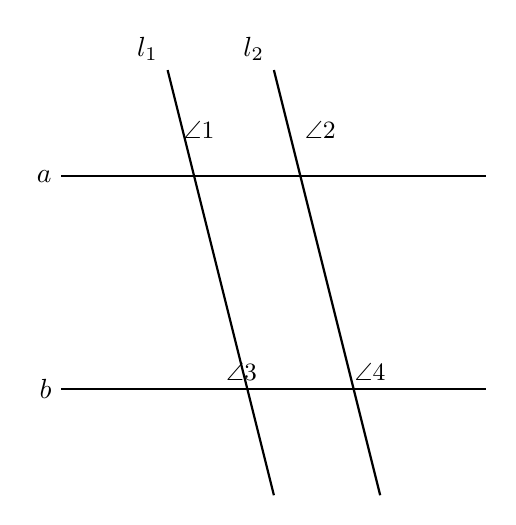
\begin{tikzpicture}[scale=0.9]
    \coordinate (A) at (-3, 1.5);
    \coordinate (B) at (3, 1.5);
    \coordinate (C) at (-3,-1.5);
    \coordinate (D) at (3,-1.5);
    \draw[thick] (A) -- (B);
    \draw[thick] (C) -- (D);
    \draw[thick] (-1.5,3) -- (0,-3);
    \draw[thick] (0,3) -- (1.5,-3);
    \node[left] at (A) {$a$};
    \node[left] at (C) {$b$};
    \node[above left] at (-1.5,3) {$l_1$};
    \node[above left] at (0,3) {$l_2$};
    \node[above left] at (-0.7,1.9) {\small $\angle 1$};
    \node[above right] at (0.3,1.9) {\small $\angle 2$};
    \node[below left] at (-0.1,-1.0) {\small $\angle 3$};
    \node[below right] at (1.0,-1.0) {\small $\angle 4$};
  \end{tikzpicture}
  \end{center}
\end{enumerate}

\vspace{10pt}
\begin{knowledgebox}[参考答案]
\begin{enumerate}[leftmargin=2em]
  \item 对顶角 $= 130°$，邻补角 $= 180° - 130° = 50°$。

  \item $a \parallel c$（或 $a$ 与 $c$ 重合）。理由：$a \perp b$，$b \perp c$，即 $a$ 与 $c$ 都垂直于 $b$。在同一平面内，过直线外一点（或同一条垂线的方向上）与已知直线垂直的直线方向相同，故 $a \parallel c$。

  \item 过 $E$ 作 $EF \parallel AB$，则 $EF \parallel CD$。$\angle ABE = \angle BEF = 40°$，$\angle CDE = \angle DEF = 60°$。$\angle BED = 40° + 60° = 100°$。

  \item 平行。$\angle 1 + \angle 2 = 110° + 70° = 180°$，同旁内角互补，两直线平行。

  \item 因为 $\angle 1 = \angle 2$，所以 $l_1 \parallel l_2$（同位角相等）。因为 $l_1 \parallel l_2$，所以 $\angle 3 + \angle 4 = 180°$（同旁内角互补）。$\angle 4 = 180° - 100° = 80°$。
\end{enumerate}
\end{knowledgebox}

\vfill
\begin{center}
\small\textcolor{gray}{本讲义仅供教学参考，例题可根据学生水平调整难度。}
\end{center}

\end{document}
